\documentclass[12pt]{article}

% Package for encoding and language support
\usepackage{indentfirst}

% \usepackage[utf8]{inputenc}
\usepackage{amsmath}
\usepackage{amssymb}
\usepackage{amsfonts}
\usepackage{geometry}
\usepackage{graphicx}
\usepackage{fancyhdr}
\usepackage{enumitem}
\usepackage{hyperref}
\usepackage{url}




% Page margins
\geometry{a4paper, margin=1in}

% Header and footer
\setlength{\headheight}{14.49998pt}
\addtolength{\topmargin}{-2.49998pt}

\pagestyle{fancy}
\fancyhf{}
\fancyhead[L]{Big-Data-Analytics HW 01}
\fancyhead[R]{Yushan Liu 2024214103}
\fancyfoot[C]{\thepage}

% Title information

\begin{document}

\begin{titlepage}
    \begin{center}
        % Insert logo
        
\includegraphics[width=5cm]{tsinghua_logo.png}\\[4cm]  % 插入图标并设置下方间距
        {\Huge Homework 1:ANOVA} \\[2cm]
        {\large Yushan Liu  \ \  Student ID: 2024214103}\\[6cm]
        {\normalsize \today}\\[1cm]
    \end{center}
\end{titlepage}

\section*{Problem 1}

One-way ANVOA is based on the following assumptions:

\begin{enumerate}
    \item \textbf{Independence of Observations}: The observations within each group and between groups must be independent of each other.
    
    \item \textbf{Normality}: The dependent variable should be approximately normally distributed for each group.
    
    \item \textbf{Homogeneity of Variances (Homoscedasticity)}: The variance of the dependent variable should be equal across the different groups being compared.
\end{enumerate}

\section*{Problem 2}

We are asked to determine if the feature "Average Age" (Col[7]) significantly varies across different group categories (Col[2]). To achieve this, we need to state the null and alternative hypotheses.

\begin{itemize}
    \item \textbf{Null Hypothesis (H$_0$)}: The average age is the same across all group categories. Mathematically, this can be written as:
    \[
    H_0: \mu_1 = \mu_2 = \mu_3 = \mu_4 = \mu_5
    \]
    Where $\mu_i$ represents the mean of the average age for category $i$ (where $i = 1, \dots, 5$).
    
    \item \textbf{Alternative Hypothesis (H$_1$)}: At least one group category has a significantly different average age compared to the others. This is expressed as:
    \[
    H_1: \exists \, i, j \ \text{such that} \ \mu_i \neq \mu_j
    \]
    This means that not all the category means are equal; at least one category has a different mean average age.
\end{itemize}

The goal of ANOVA is to test whether the null hypothesis can be rejected, indicating that there is a significant difference in the average age across the different group categories.


\section*{Problem 3}

\subsection*{(a) Empirical PDF and Normality Test}

We use the following Python code to plot the empirical probability density function (PDF) of the "Average Age" (Col[7]) and perform the Shapiro-Wilk test to assess the normality of the data:

\begin{verbatim}
    import pandas as pd
    import numpy as np
    import seaborn as sns
    import matplotlib.pyplot as plt
    from scipy import stats

    data = pd.read_excel('data.xlsx')
    col_7 = data.iloc[:, 6]  

    sns.kdeplot(col_7, bw_adjust=0.5)
    plt.title('Empirical PDF of Col[7]')
    plt.xlabel('Average Age')
    plt.ylabel('Density')
    plt.grid()
    plt.show()

    statistic, p_value = stats.shapiro(col_7) 
    print(f'Statistic: {statistic}, p-value: {p_value}')

    alpha = 0.05
    if p_value > alpha:
        print("Fail to reject null hypothesis.")
    else:
        print("Reject null hypothesis.")

\end{verbatim}

In this code, we first load the data from the Excel file and extract the "Average Age" column (Col[7]). We then plot the empirical PDF of the data using a kernel density estimate (KDE) plot. Finally, we perform the Shapiro-Wilk test to assess the normality of the data. The test outputs the test statistic and p-value, which we use to determine whether the data is normally distributed. The test normality by plot is as follows:

\begin{figure}[h]
    \centering
    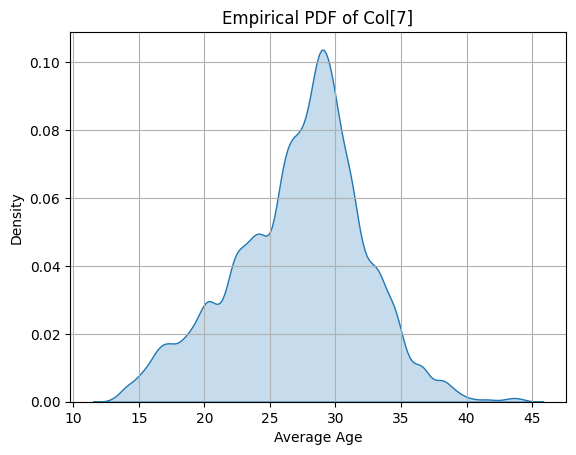
\includegraphics[width=0.68\textwidth]{image/output1.png}  
    \label{fig:Output for Normality Test}
\end{figure}

According to the Shapiro-Wilk test, the p-value is less than 0.05, indicating that we reject the null hypothesis of normality. Therefore, the "Average Age" data does not follow a normal distribution.

\subsection*{(b) Normality and Homogeneity of Variance Tests}


To test the homogeneity of variance assumption, we can use Levene's test. The following Python code demonstrates how to perform Levene's test to assess the homogeneity of variance across the different group categories:

\begin{verbatim}
    import pandas as pd
    from scipy import stats
    from statsmodels.stats.proportion import proportions_ztest

    # Read data
    data = pd.read_excel('data.xlsx')

    # Extract column 7 and categories
    col_7 = data.iloc[:, 6]  # 7th column
    categories = data['群类别']  # Assuming the category column is named 'category'

    # Test normality for each category
    for i in range(1, 6):  # Assuming categories are labeled from 1 to 5
        group = col_7[categories == i]
        statistic, p_value = stats.shapiro(group)  # Shapiro-Wilk test
        print(f'Category {i}: Statistic={statistic}, p-value={p_value}')
        if p_value > 0.05:
            print(f'Category {i} appears to be normally distributed')
        else:
            print(f'Category {i} does not appear to be normally distributed')

    # Test homogeneity of variances
    groups = [col_7[categories == i] for i in range(1, 6)]
    stat, p_value_var = stats.levene(*groups)  # Levene's test
    print(f'Levene’s test: Statistic={stat}, p-value={p_value_var}')
    if p_value_var > 0.05:
        print('Homogeneity of variances is assumed (fail to reject H0)')
    else:
        print('Homogeneity of variances is not assumed (reject H0)')

\end{verbatim}

The code first reads the data from Col[7] and the category labels. For each category (i = 1, ..., 5), the Shapiro-Wilk test is applied to assess the normality of the data within that category. If the p-value from the test is greater than 0.05, we cannot reject the null hypothesis, meaning the data appears to follow a normal distribution. Otherwise, the data does not follow a normal distribution.

Next, the Levene's test is performed to check the homogeneity of variances across the five categories. A p-value greater than 0.05 indicates that the assumption of equal variances holds, while a smaller p-value suggests significant variance differences between categories.

By running the code, we can know that even if in the same category, the data does not follow a normal distribution. The homogeneity of variances is not assumed. The output of the code is as follows:

\begin{verbatim}
    Category 1: Statistic=0.9889177019317387, p-value=0.0010068367942714259
    Category 1 does not appear to be normally distributed (reject H0)
    Category 2: Statistic=0.9866028570038597, p-value=0.006910100085120613
    Category 2 does not appear to be normally distributed (reject H0)
    Category 3: Statistic=0.9894059994096522, p-value=0.15584690304319565
    Category 3 appears to be normally distributed (fail to reject H0)
    Category 4: Statistic=0.9838728658098733, p-value=0.00011372764101030563
    Category 4 does not appear to be normally distributed (reject H0)
    Category 5: Statistic=0.9546671623519278, p-value=4.544352530487091e-13
    Category 5 does not appear to be normally distributed (reject H0)
    Levene’s test: Statistic=61.01927977094263, p-value=9.677355333795493e-49
    Homogeneity of variances is not assumed (reject H0)

\end{verbatim}

\subsection*{(c) One-Way ANOVA Test}

To determine whether the average age significantly varies across the different group categories, we can perform a one-way ANOVA test. The following Python code demonstrates how to conduct the ANOVA test using the \texttt{scipy.stats} library:

\begin{verbatim}
    import pandas as pd
    from scipy import stats
    import seaborn as sns
    import matplotlib.pyplot as plt


    data = pd.read_excel('data.xlsx')
    col_7 = data.iloc[:, 6]
    categories_col_2 = data.iloc[:, 1]

    groups = [col_7[categories_col_2 == category] for category in categories_col_2.unique()]


    stat, p_value = stats.f_oneway(*groups)
    print(f'ANOVA test statistic: {stat}, p-value: {p_value}')

    plt.figure(figsize=(10, 6))
    sns.boxplot(x=categories_col_2, y=col_7)
    plt.title('Boxplot of Col[7] Across Categories in Col[2]')
    plt.xlabel('Category (Col[2])')
    plt.ylabel('Values of Col[7]')
    plt.grid()
    plt.show()

    alpha = 0.05
    if p_value > alpha:
        print("No significant difference between the means of the groups.")
    else:
        print("Significant difference between the means of the groups.")
\end{verbatim}


We performed a one-way ANOVA test to compare the means of Col[7] across different categories in Col[2]. The ANOVA test resulted in a test statistic of \texttt{stat} and a p-value of \texttt{p\_value}. In addition, we plotted a boxplot to visualize the distribution of Col[7] across different categories in Col[2], which provides an intuitive view of the differences in means and variances between groups. 


The output of the code is as follows, we can know that the p-value is less than 0.05, indicating that we reject the null hypothesis of equal means across the groups. Therefore, there is a significant difference in the average age across the different group categories.

\begin{figure}[h]
    \centering
    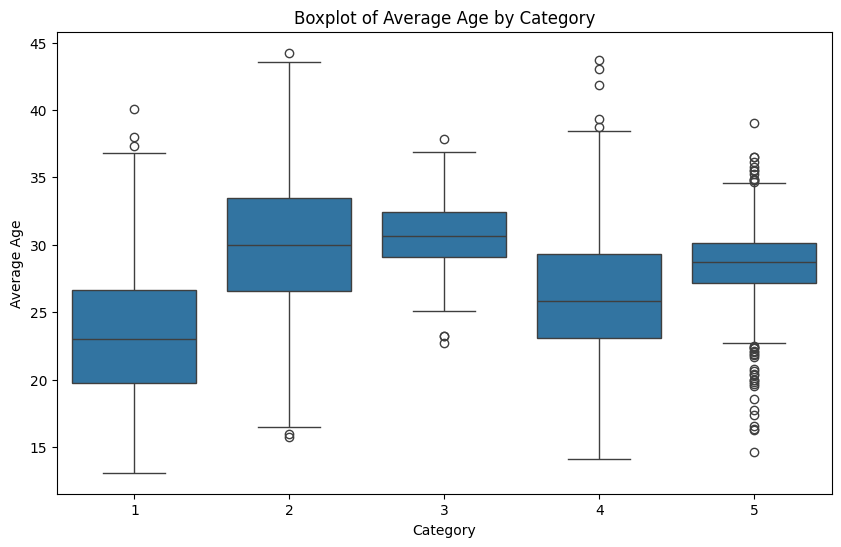
\includegraphics[width=0.8\textwidth]{image/output2.png}  
    \label{fig:Output for ANOVA test}
\end{figure}

\section*{Problem 4}

\newpage
\begin{thebibliography}{99}

    \bibitem{CCS229LectureNotes}
    Andrew Ng, Tengyu Ma. \textit{CCS 229 Lecture Notes}. Stanford University, 2023. Available online at: \url{{https://cs229.stanford.edu/}}
    
    \bibitem{ConvexOptimization}
    Stephen Boyd, Lieven Vandenberghe. \textit{Convex Optimization}. Cambridge University Press, 2004.
    
    \bibitem{ChatGPT}
    OpenAI. \textit{ChatGPT: A Conversational AI}. 2023. Available online at: \url{{https://www.openai.com/chatgpt}}
    
    \bibitem{chung2001stochastic}
    K. L. Chung. \textit{Stochastic Processes}. 2nd ed. Springer, 2001.

    \end{thebibliography}
    
\end{document}
